\usepackage[T1]{fontenc}
\usepackage{lmodern,amsmath,amssymb,booktabs,array,graphicx,tikz}
\usetikzlibrary{arrows.meta,positioning}
\definecolor{ink}{HTML}{253443}
\definecolor{accent}{HTML}{1474A8}
\definecolor{muted}{HTML}{647180}
\definecolor{bank}{HTML}{CB7037}
\newcommand{\code}[1]{\nolinkurl{#1}}
\newcommand{\point}[1]{\par\medskip\textbf{#1}\par}
\newcommand{\refpaper}[2]{\href{#1}{#2}}
\newcommand{\E}{\mathbb{E}}
\newcommand{\R}{\mathbb{R}}
\newcommand{\sg}{\operatorname{sg}}
\newcommand{\softmax}{\operatorname{softmax}}
\newcommand{\architecture}{%
\begin{center}
\resizebox{.96\linewidth}{!}{%
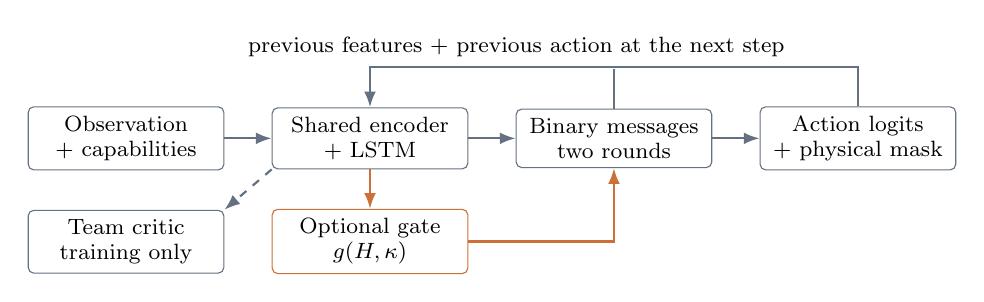
\begin{tikzpicture}[box/.style={draw=muted,rounded corners=2pt,align=center,
 minimum height=.65cm,text width=2.25cm,font=\fontsize{8}{9}\selectfont},
 arrow/.style={-{Latex[length=2mm]},draw=muted,thick}]
\node[box] (obs) {Observation\\+ capabilities};
\node[box,right=6mm of obs] (rec) {Shared encoder\\+ LSTM};
\node[box,right=6mm of rec] (com) {Binary messages\\two rounds};
\node[box,right=6mm of com] (act) {Action logits\\+ physical mask};
\draw[arrow] (obs)--(rec); \draw[arrow] (rec)--(com); \draw[arrow] (com)--(act);
\node[box,below=5mm of rec,draw=bank] (gate) {Optional gate\\$g(H,\kappa)$};
\draw[arrow,draw=bank] (rec)--(gate);
\draw[arrow,draw=bank] (gate.east)-|(com.south);
\node[box,below=5mm of obs] (critic) {Team critic\\training only};
\draw[arrow,dashed] (rec.south west)--(critic.north east);
\draw[arrow] (act.north)--++(0,.5)-|node[pos=.35,above,font=\fontsize{8}{9}\selectfont]{previous features + previous action at the next step}(rec.north);
\draw[draw=muted,thick] (com.north)--++(0,.5);
\end{tikzpicture}}
\end{center}}
